\section{UNet+++ Method}
After UNet and UNet++, we also try UNet+++\cite{unet_ppp},
which was developed and published in 2020 and maybe the latest UNet-like deep learning network.
In the following sections, we first briefly introduce UNet+++ according to the paper, and then introduce our training methods and results.

\subsection{Network description}
In image segmentation, Combining multi-scale features is one of important factors for accurate segmentation.
In recent deep learning network like UNet and UNet++, feature maps in different scale explore distinctive information. Lowlevel detailed feature maps capture rich spatial information, 
while high-level semantic feature maps embody position information. 
Nevertheless, these exquisite signals may be gradually diluted when progressively down- and up-sampling.
However, by implementing full-scale skip connections, UNet+++ can make full use of the multi-scale features, incorporating low-level details with high-level semantics from feature maps in different scales. 
The following image displays simplified overviews of UNet, UNet++ and UNet+++. The image is from \cite{unet_ppp}

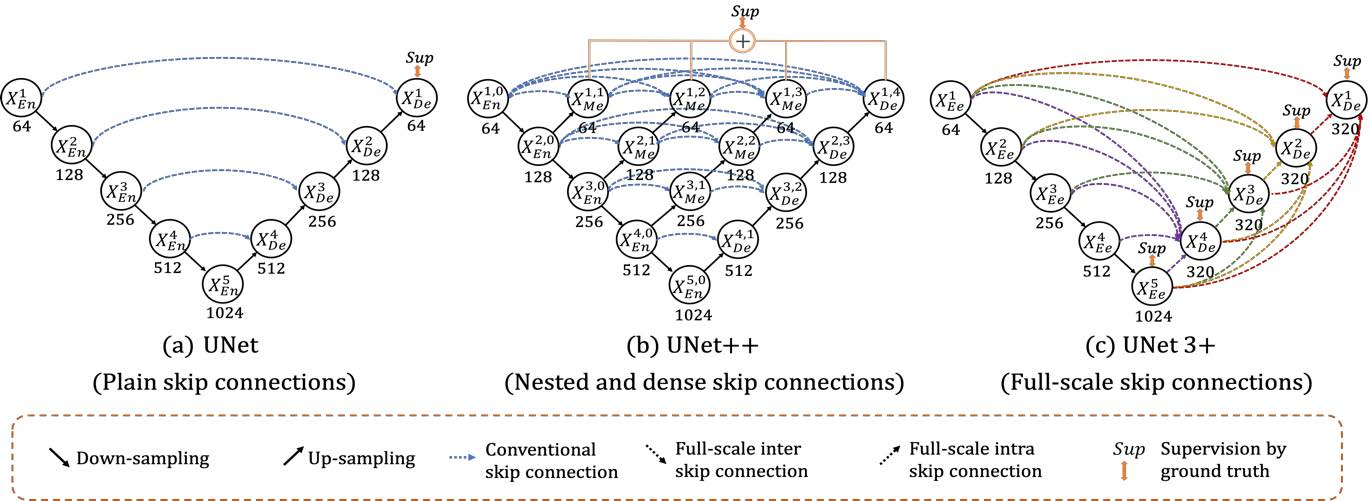
\includegraphics[width=\linewidth]{figuras/UNet+++.jpg}

\subsection{Algorithm}
We use Pytorch to train UNet+++, so we use Pytorch's loss function and optimizer.

In details, because the result picture only have two class 0,1 per pixel, we use loss function BCEWithLogitsLoss, it combines a Sigmoid layer and the BCELoss. 
BCELoss is a criterion that measures the Binary Cross Entropy between the target and the output, the formula is:
\[\begin{aligned}
    &\bm{l}(\bm{x}, \bm{y})=\{l_1, \cdots, l_N\}^T, \\
    &l_n=-w_n[y_n\cdot\log{x_n}+(1-y_n)\cdot\log{(1-x_n)}]
\end{aligned}\]
Where N is the batch size. BCEWithLogitsLoss is more numerically stable than using a plain Sigmoid followed by a BCELoss as, 
by combining the operations into one layer, we take advantage of the log-sum-exp trick for numerical stability.

We use Adam algorithm as optimizer. Actually we test Adam, RMSprop, SGD and we find that Adam performs best.

\subsection{Experimental and Results}
We use the given dataset to train and test the network, the learning rate is the default value(0.001) of torch.optim.Adam.
Because the network is complex, we can only set batch size to 1, otherwise the GPU memory is not enough.

We test the relationship between epoch and the accuracy of test data, in order to find the best epoch value. In the test, the value of epoch range from 1 to 40. 
In each iteration, we test the current model on test dataset, and record the accuracy. The result is given in the following image.

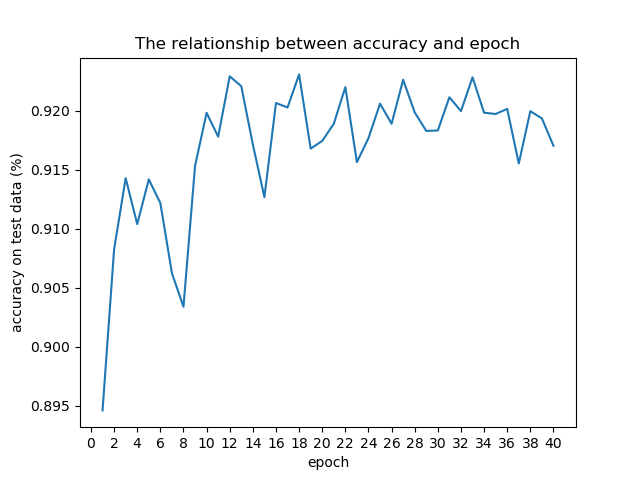
\includegraphics[width=\linewidth]{figuras/epoch_accuracy.png}

The image shows that as the epoch value increase, the accuracy first increase rapidly and than decrease slowly, 
which means that when epoch is too large, it becomes overfitting.
The best accuracy is 0.923, with the epoch value 18


